\section{Kostenschätzung}

Das finden des besten Plans geschieht über die Kostenberechnung. Nur der Plan mit den niedrigsten Kosten ist der optimale Plan. Wie in System R wird davon ausgegangen, dass ein optimaler Plan aus optimalen Teilplänen besteht. Auch dieser Prototyp folgt damit dem Optimalitätsprinzip von Bellman \cite{Bellman:1957}.

Zur Ermittlung der Kosten können unterschiedliche Parameter herangezogen werden. Beispielsweise kann die CPU-Zeit, der I/O-Zugriff und andere Parameter genutzt werden. Für den Prototypen wurde eine möglichst einfache Form der Kostenschätzung auf Basis der Kardinalitäten und Selektivitäten implementiert.

In der konkreten Implementierung wird davon ausgegangen, die Kosten direkt in Zusammenhang mit der Kardinalität stehen und 1:1 umgerechnet werden können. So sind die Kosten für das Lesen einer Basis-Relation mit der Kardinalität von 100 auch 100. Findet ein JOIN zwischen zwei Relationen mit einer Kardinalität von je 50 statt und einer Selektvitität von 0.1 ist die Kardinalität des Join Knotens 250 und damit die Kosten für den Join 250. Nimmt man die Kosten für das lesen der beiden Relationen hinzu (je 50), ergeben sich die Kosten für den gesamten Teilbaum. Dieses Vorgehen setzt einen Bottom-up-Ansatz voraus. Zuerst müssen alle Teilbäume berechnet werden, bevor der gesamte Baum berechnet werden kann.

\subsection{Implementierung der Kostenfunktion}


\begin{figure}[ht]
  \centering
  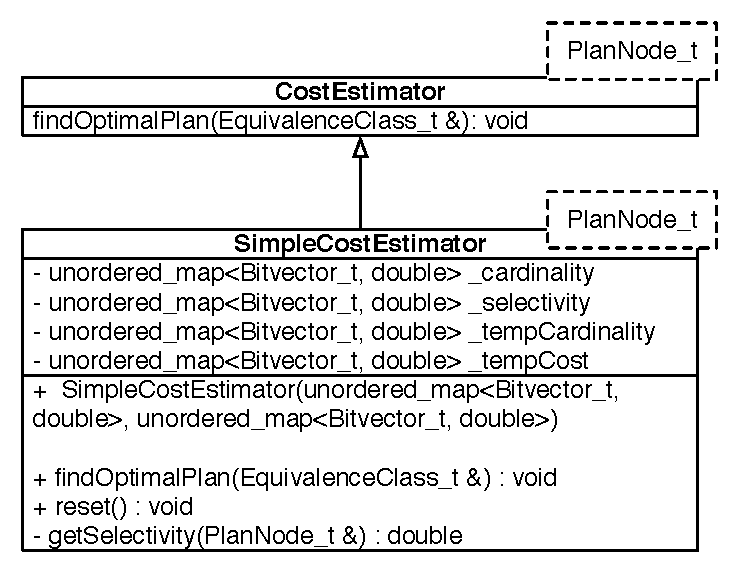
\includegraphics[width=0.75\textwidth]{04_Implementierung/00_media/ClassCostEstimation.pdf}
  \caption{Klassendiagramm: Kostenschätzung}
  \label{ClassCostEstimation}
\end{figure}



Die konkrete Implementierung der Kostenfunktion wird in der Klasse \texttt{Simple\-Cost\-Estimator} vorgenommen. In ihrem Konstrukor wird die Kardinalität und die Selektvität von Basis-Relationen und Join-Kanten übergeben. Sie stammen aus der Konfiguration und sind die Grundlage der Berechnung. Die Klasse erfüllt das Interface \texttt{Cost\-Estimator}, das die Methode \texttt{find\-Optimal\-Plan(Equivalence\-Class\_t \&)} vorgibt. Dies ist in Abb. \ref{ClassCostEstimation} zu sehen.

Die Hilfsmethode  \texttt{get\-Selectivity(Plan\-Node\_t \&)} ermittelt die Selektivität für einen Planknoten.


Die Kostenberechnung wird rekursiv durchgeführt. Wie in \ref{PseudocodeCostEstimator} zu sehen ist, wird für jeden Planknoten, der in der Äquivalenzklasse vorhanden ist, zuerst geprüft, ob es sich um einen \texttt{SCAN} handelt. Wie zuvorbeschrieben existieren zwei Operatoren \texttt{JOIN} und \texttt{SCAN}. Es ist nicht möglich, dass einem \texttt{SCAN} ein \texttt{JOIN} untergeordnet ist. 

Somit sind die Kosten für einen \texttt{SCAN} nach unserem Kostenmodell gleich der Kardinalität des \texttt{SCAN}-Planknoten. Falls es sich um keinen \texttt{SCAN} handelt, wird geprüft, ob die linke und der rechte Äuqivalenzklasse einen optimalen Planknoten gefunden haben. Wenn das nicht der Fall ist, wird die Suche nach diesen angestossen und somit der Rekursion gestartet. Nachdem die optimalen Planknoten für die untergeordneten Äquivalenzklassen gefunden sind, kann die Kardinalität sowie die Kosten für den akteullen Knoten berechnet werden. Falls die Kosten niedriger sind als die bisher bekannten Kosten für den bisher optimalen Plan, wird der beste Plan neu gesetzt und die optimalen Kosten und die Kardinaltität des Äquivalenzknotens angepasst.



\begin{algorithm}[ht]
\SetAlgoLined
\SetKwFunction{findOptimalPlan}{findOptimalPlan}
\SetKwProg{myalg}{Algorithm}{}{}

\myalg{\findOptimalPlan{EquivalenceClass eq}}{
    \For{PlanNode p in eq.PlanNodes}{
        \If{p.operator == SCAN}{
            eq.best = p
            
            eq.costs = p.cardinality
            
            eq.cardinality = p.cardinality
            
            return
        }
        
        \If{p.left.best == NULL}{
            findOptimalPlan(p.left)
        }
        \If{p.right.best == NULL}{
             findOptimalPlan(p.right)
        }
        
        p.cardinality = p.left.cardinality * p.right.cardinality * p.selectivity
        
        p.cost = p.left.cost + p.right.cost + p.cardinality
        
        \If{p.cost < eq.cost OR eq.cost == NULL}{
            eq.cost = p.cost
            
            eq.cardinality = p.cardinality
            
            eq.best = p
        }
    }
}
\label{PseudocodeCostEstimator}
\caption{Kostenfunktion: SimpleCostEstimator}
\end{algorithm}


\subsection{Erweiterbarkeit der Kostenfunktion}
Diese Implementierung ist nur eine starke Vereinfachung. Sie bezieht nur sehr einfache Parameter in die Berechnung ein. Keine komplexen Kostenfunktionen wurden implementiert. Dank der Modularität des Prototypen ist es möglich, neue, akkuratere Kostenfunktionen zu erstellen und diese auch zu implementieren. Dafür muss ausschließlich das Interface \texttt{Cost\-Estimator} erfüllt werden, das bereits in Abb. \ref{ClassCostEstimation} vorgestellt wurde.
